\documentclass[report.tex]{subfiles}
\begin{document}
\section{Baseline with Middleware (90 pts)}\label{exp3}

%In this set of experiments, you will have to use 1 load generator VM and 1 memcached server, measuring how the throughput of the system changes when increasing the number of clients. Scaling virtual clients inside memtier has to be done as explained in the previous sections. Plot both throughput and response time as measured on the middleware.

In this set of experiments the impact of the number of clients on the  performance of the system is studied when using 3 load generating VMs and 1 \emph{memcached} server. 

All measurements are validated using the interactive law, which describes the relationship between throughput $X$ and response time $R$ in a closed system with $N$ clients where each client has a client thinking time of $Z$ (Eq. \ref{ilaw}). For all experiments a client thinking time of $Z = 0$ is used. The interactive law is expected to hold for all experiments.

\begin{equation}\label{ilaw}
R = \frac{N}{X} - Z
\qquad\qquad\qquad\qquad
Error = R_{client} - (\frac{N}{X_{mw}}  - Z)
\end{equation}

However, the interactive law cannot be applied directly to validate the MW throughput and response time measurements.
This is due to the fact that the middleware cannot measure the time a request needs for the transport over the network between client and MW. This results in a shorter response time measurement in the middleware than the actual response time measured on the client.
Hence when using the middleware response time, this would result in a throughput that is higher than the measured throughput.
To circumvent this issue while still being able to use the interactive law as a sanity check for the collected data, the response time as measured on the client is used instead. In addition a manual check was performed to verify that the response time differences between client and middleware measurements is approximately the round trip time between client VM and middleware VM: $R_{client} - R_{mw} \approx rtt$.


\subsection{One Middleware}\label{exp31}

Three load generating VMs are connected to one middleware handling requests for a single server. 
The number of clients is varied between 6 and 288 depending on the saturation of the system with 8, 16, 32 and 64 worker threads inside the 
middleware for both a read-only and write-only workload. The details of the configuration are shown in the table below.
The interactive law was checked and holds for all experiments in this section (Tab. \ref{exp31_ilaw})

\begin{center}
	\scriptsize{
		\begin{tabular}{|l|c|}
			\multicolumn{2}{l}{3 client VMs, 1 middleware VM and 1 server VM}\\
			%\hline Number of servers                & 1                        \\ 
			%\hline Number of client machines        & 3                        \\ 
			\hline Instances of memtier per machine & 1                        \\ 
			\hline Threads per memtier instance     & 2                        \\
			\hline Virtual clients per thread       & [1, 2, 4, 8, 12, 16, 24, 32, 48] \\ 
			\hline Workload                         & Write-only and Read-only \\
			%\hline Multi-Get behavior               & N/A                      \\
			%\hline Multi-Get size                   & N/A                      \\
			%\hline Number of middlewares            & 1                        \\
			\hline Worker threads per middleware    & [8, 16, 32, 64]                  \\
			%\hline Repetitions                      & 3 or more (at least 1 minute each)                \\ 
			\hline 
		\end{tabular}
	} 
\end{center}

\begin{figure}[H]
	\begin{subfigure}[b]{.499\linewidth}
		\centering
		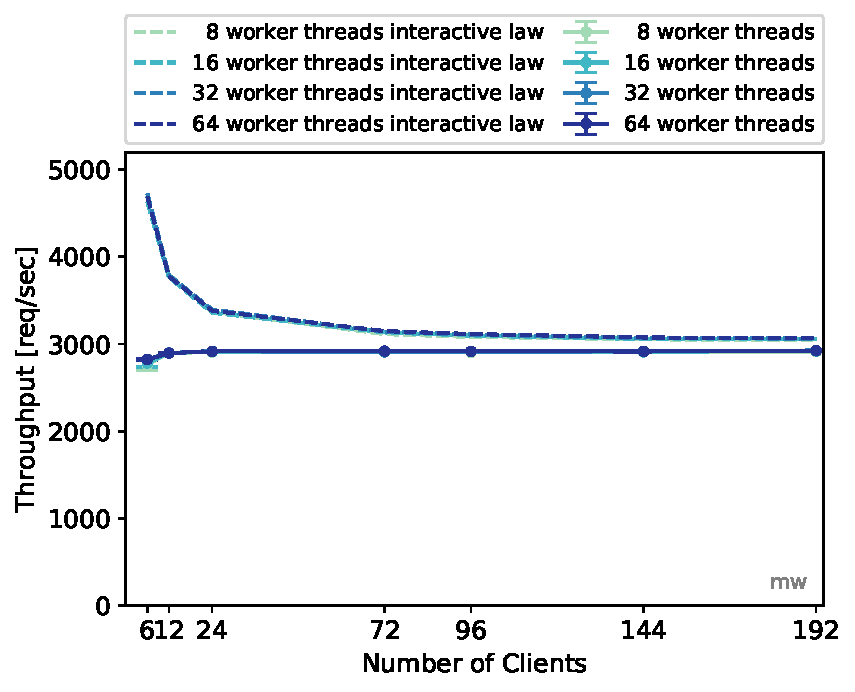
\includegraphics[width=\linewidth]{data/exp31_ro_tp_nc_w.pdf}
	\end{subfigure}\hfill
	\begin{subfigure}[b]{.499\linewidth}
		\centering
		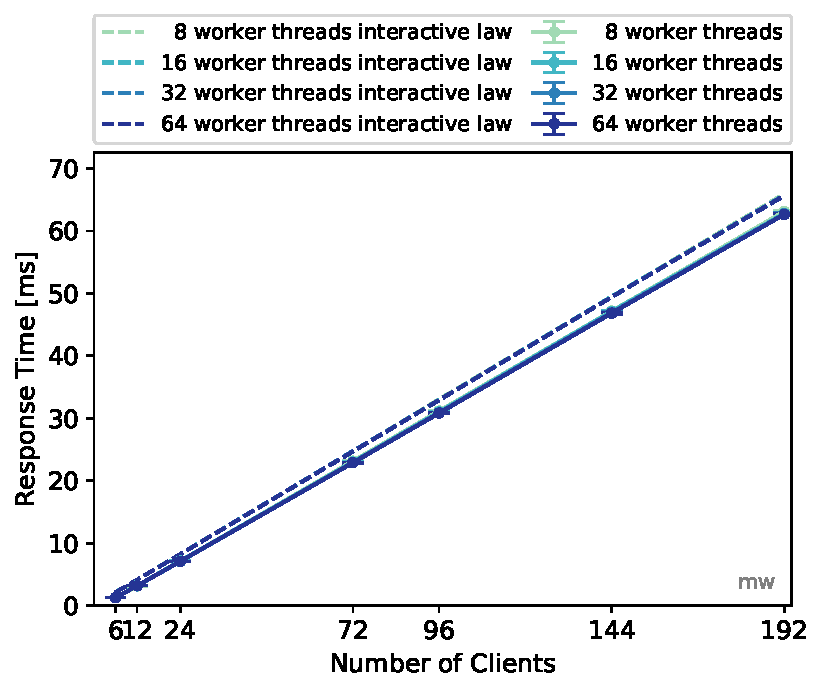
\includegraphics[width=\linewidth]{data/exp31_ro_rt_nc_w.pdf}
	\end{subfigure}%
	\caption{Throughput and response time in read-only workload for the system with 1 MW as a function of number of clients. The sample standard deviation over the repetitions is used as the error metric to show that the measurements are stable.}\label{exp31_ro_tp_nc}
\end{figure}

\begin{figure}[H]
	\begin{subfigure}[b]{.499\linewidth}
		\centering
		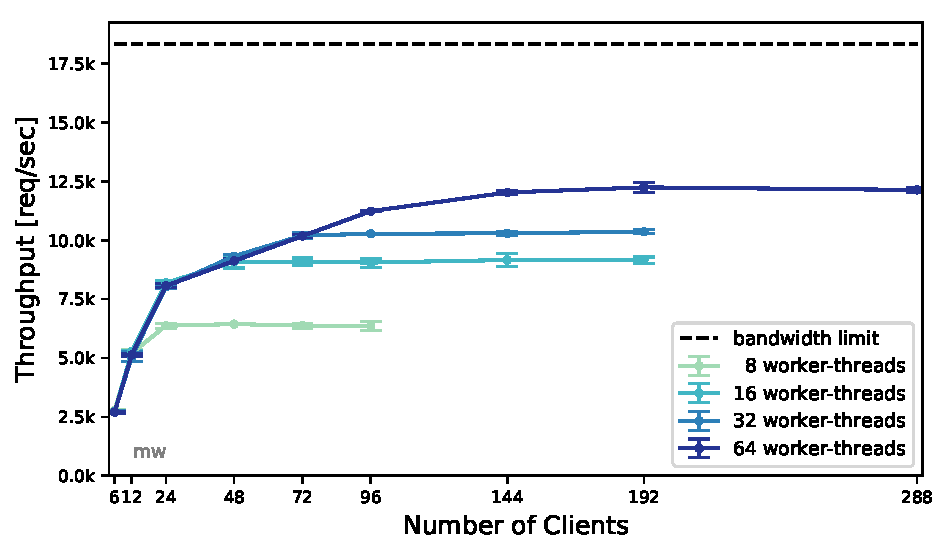
\includegraphics[width=\linewidth]{data/exp31_wo_tp_nc_w.pdf}
	\end{subfigure}\hfill
	\begin{subfigure}[b]{.499\linewidth}
		\centering
		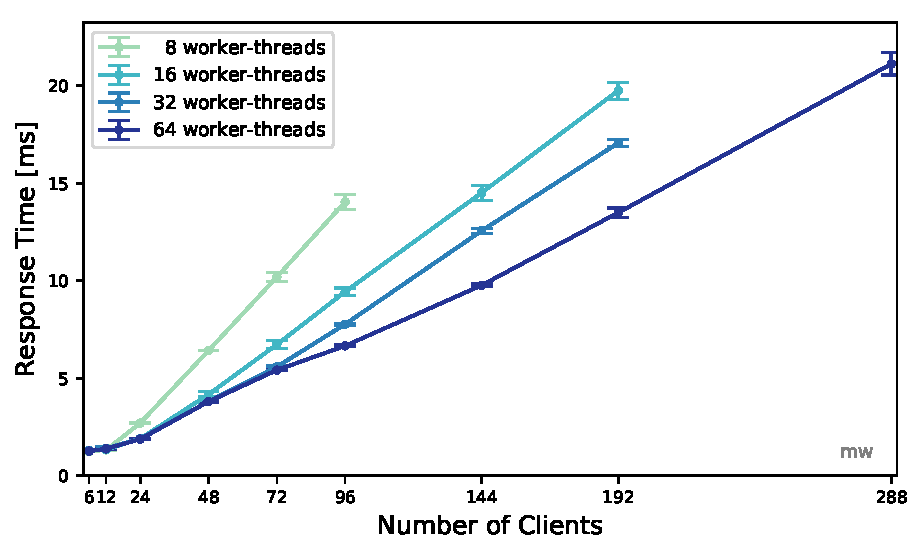
\includegraphics[width=\linewidth]{data/exp31_wo_rt_nc_w.pdf}
	\end{subfigure}
\caption{Throughput and response time in write-only workload for the system with 1 MW as a function of number of clients. The sample standard deviation over the repetitions is used as the error metric to show that the measurements are stable.}\label{exp31_wo_tp_nc}
\end{figure}

\subsubsection{Explanation}

\paragraph{Read-Only Workload}


As described in section \ref{exp2}, the read-only workload with a single \emph{memcached} server VM and values of size 4096B is bound to around 3000 ops/sec by the upload bandwidth of the server VM. This phenomena is also clearly visible in figure \ref{exp31_ro_tp_nc} when using a single middleware in between 3 client VMs and a server VM. Consequently the point of throughput saturation of a read-only workload is reached already with 6 clients, independent of the number of worker-threads. This also manifests itself in the response time that increases linearly in the number of clients due to the extended waiting period on the server VM.

In the following it is analysed how this network bandwidth bottleneck manifests itself in the middleware measurements. 
As long as the number of clients is less than the number of workers per MW, the request queue in the middleware is empty (Fig. \ref{exp31_ro_q}). This is because the number of clients in a closed system limit the number of requests that can be in the MW at the same time. 
So when there are more worker-threads than possible requests in the system, every request placed in the queue is processed immediately by one of the idle workers. This is a fact that holds independently of the network bottleneck. 

Figure \ref{exp31_ro_tp_nc} shows that the response time is not affected by the number of worker-threads because already using 8 workers is enough in combination with 12 clients to reach the network bottleneck. So adding more workers cannot improve the throughput. 
However, the response time increases in the number of clients because the number of requests per second that can be transported from the server VM to the MW remains fixed. Consequently with a greater user-load, requests need to wait longer in some part of the system before the bottleneck, leading to a longer response time.
This also manifests itself in the different components of the response time.
The queue waiting time and the server service time are the two dominant factors of the response time as measured on the client while the network-, the net-thread decoding- and worker-thread processing time are negligibly small  (Fig. \ref{exp31_ro_rtcomp}). As the number of worker increases, requests spend less time in the queue and instead stay longer on the server VM where they are waiting in front of the network bottleneck. 
So the number of workers does not influence the response time but it influences if the requests are queued in the middleware or on the server (Fig. \ref{exp31_ro_rtcomp}).

The server service time increases up to the point where are all workers are busy and the queue starts to fill up. Afterwards it remains constant because the number of workers in the middleware limit the number of requests that can be concurrently at the server VM and hence need to be sent through the network bottleneck. (Fig. \ref{exp31_ro_sst})


\begin{figure}[H]
	\begin{subfigure}[b]{.33\linewidth}
		\centering
		\includegraphics[width=\linewidth]{data/exp31_ro_queue_nc_w.pdf}
		\caption{}\label{exp31_ro_q}
	\end{subfigure}\hfill
	\begin{subfigure}[b]{.33\linewidth}
		\centering
		\includegraphics[width=\linewidth]{data/exp31_ro_sst_nc_w.pdf}
		\caption{}\label{exp31_ro_sst}
	\end{subfigure}\hfill
	\begin{subfigure}[b]{.33\linewidth}
		\centering
		\includegraphics[width=\linewidth]{data/exp31_ro_rt_component_w.pdf}
		\caption{}\label{exp31_ro_rtcomp}
	\end{subfigure}
	\caption{Length of queue and server service time as a function of number of clients with sample standard deviation over the repetitions as the error metric and client response time components for 96 clients in a read-only workload with 1 MW.}
\end{figure}


\paragraph{Write-Only Workload}


The data in figure \ref{exp31_wo_tp_nc} indicates that the throughput saturates for a different number of clients when varying the number of worker-threads. This is because there is a trade-off between server service time and queueing time in the MW controlled by the number of workers. For fewer workers, requests start to queue up already with a smaller number of clients because the number of worker-threads controls how many requests can be sent to the server concurrently. However with more requests at the server concurrently, the server also has a longer server service time for each of them.
The throughput saturation for 8 workers is reached at 24 clients, for 16 workers at 48 clients, for 32 workers at 72 clients and for 64 workers at 144 clients.

As the user-load is increased, eventually the waiting time in the queue becomes the dominant factor in the response time for every number of worker-threads. This is because when all workers are busy waiting for a response from the server,  each new request remains longer in the queue.
This becomes evident in the decomposition of the response time in figure \ref{exp31_wo_component_nc}.
The component utilization figure \ref{exp31_wo_util} shows that the bottleneck in the system is the number of worker-threads that are waiting concurrently for a response of the server. This suggests that increasing the number of worker-threads would further benefit the throughput. However, the increasing server service time for an individual request with a larger number of worker-threads poses a limit on this throughput increase.
When there are more clients than worker-threads, the number of requests in the queue is approximately equal to the difference between number of clients and number of worker-threads.
As in the read-only workload the net-thread decoding and worker-thread processing time remain negligible factors in the response time.


\begin{figure}[H]
	\begin{subfigure}[b]{.499\linewidth}
		\centering
		\includegraphics[width=\linewidth]{data/exp31_wo_queue_nc_w.pdf}
	\end{subfigure}\hfill
	\begin{subfigure}[b]{.499\linewidth}
		\centering
		\includegraphics[width=\linewidth]{data/exp31_wo_sst_nc_w.pdf}
	\end{subfigure}\hfill
	\caption{Queue length and average server service time per request as a function of number of clients for a write-only workload in a system with 1 MW. Both graphs show the sample standard deviation over the repetitions as error metric.}\label{exp31_wo_queue_sst_nc}
\end{figure}

\begin{figure}[H]
	\begin{subfigure}[b]{.499\linewidth}
		\centering
		\includegraphics[width=\linewidth]{data/exp31_wo_util_nc_w16.pdf}
		\caption{16 worker-threads}
	\end{subfigure}\hfill
	\begin{subfigure}[b]{.499\linewidth}
		\centering
		\includegraphics[width=\linewidth]{data/exp31_wo_util_nc_w64.pdf}
		\caption{64 worker-threads}
	\end{subfigure}\hfill
	\caption{Utilization $\frac{\text{busy time}}{\text{total time}}$ as a function of number of clients in a write-only workload with 1 MW.}\label{exp31_wo_util}
\end{figure}

\begin{figure}[H]
	\begin{subfigure}[b]{.499\linewidth}
		\centering
		\includegraphics[width=\linewidth]{data/exp31_wo_component_nc_w16.pdf}
		\caption{16 worker-threads}
	\end{subfigure}\hfill
	\begin{subfigure}[b]{.499\linewidth}
		\centering
		\includegraphics[width=\linewidth]{data/exp31_wo_component_nc_w64.pdf}
		\caption{64 worker-threads}
	\end{subfigure}\hfill
	\caption{Response time components as a function of number of clients for SET requests with 1 MW.}\label{exp31_wo_component_nc}
\end{figure}


\subsection{Two Middlewares}\label{exp32}


In this set of experiments, 3 load generating VMs are connected to 2 MWs handling requests for a single server. 
The number of clients is varied between 6 and 384 depending on the saturation of the system with 8, 16, 32 and 64 worker-threads 
per MW for both a read-only and write-only workload. The details of the configuration are shown in the table below.
The interactive law was checked and holds for all experiments in this section (Tab. \ref{exp32_ilaw})

\begin{center}
	\scriptsize{
		\begin{tabular}{|l|c|}
			\multicolumn{2}{l}{3 client VMs, 2 middleware VMs and 1 server VM}\\
			%\hline Number of servers                & 1                        \\ 
			%\hline Number of client machines        & 3                        \\ 
			\hline Instances of memtier per machine & 2                        \\ 
			\hline Threads per memtier instance     & 1                        \\
			\hline Virtual clients per thread       & [1, 2, 4, 8, 12, 16, 24, 32, 48, 64] \\ 
			\hline Workload                         & Write-only and Read-only \\
			%\hline Multi-Get behavior               & N/A                      \\
			%\hline Multi-Get size                   & N/A                      \\
			%\hline Number of middlewares            & 2                        \\
			\hline Worker threads per middleware    & [8, 16, 32, 64]                  \\
			%\hline Repetitions                      & 3 or more (at least 1 minute each)                \\ 
			\hline 
		\end{tabular}
	} 
\end{center}


\begin{figure}[H] 
\begin{subfigure}{\linewidth}
	\begin{subfigure}[b]{.49\linewidth}
		\centering
		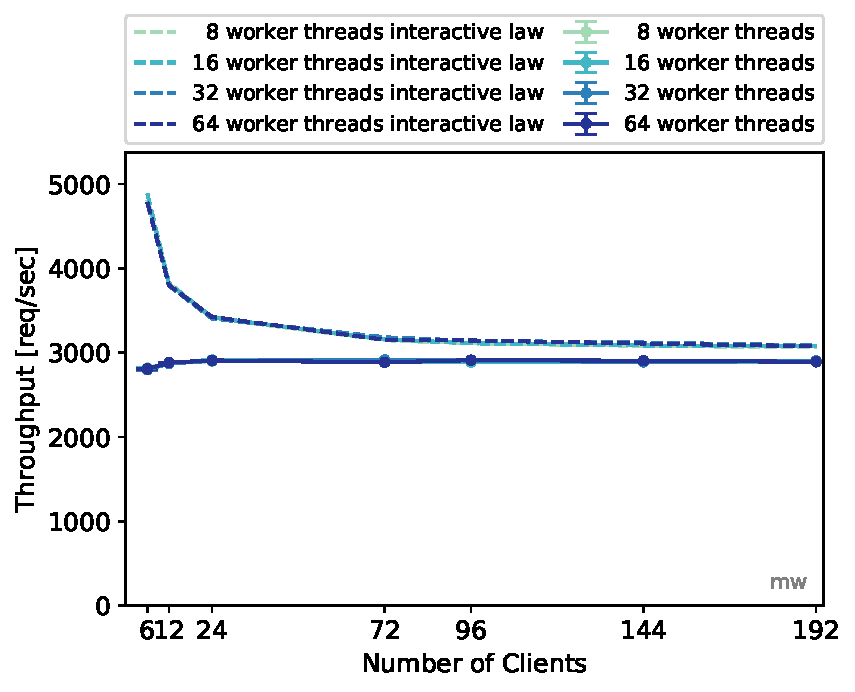
\includegraphics[width=\linewidth]{data/exp32_ro_tp_nc_w.pdf}
	\end{subfigure}\hfill
	\begin{subfigure}[b]{.49\linewidth}
		\centering
		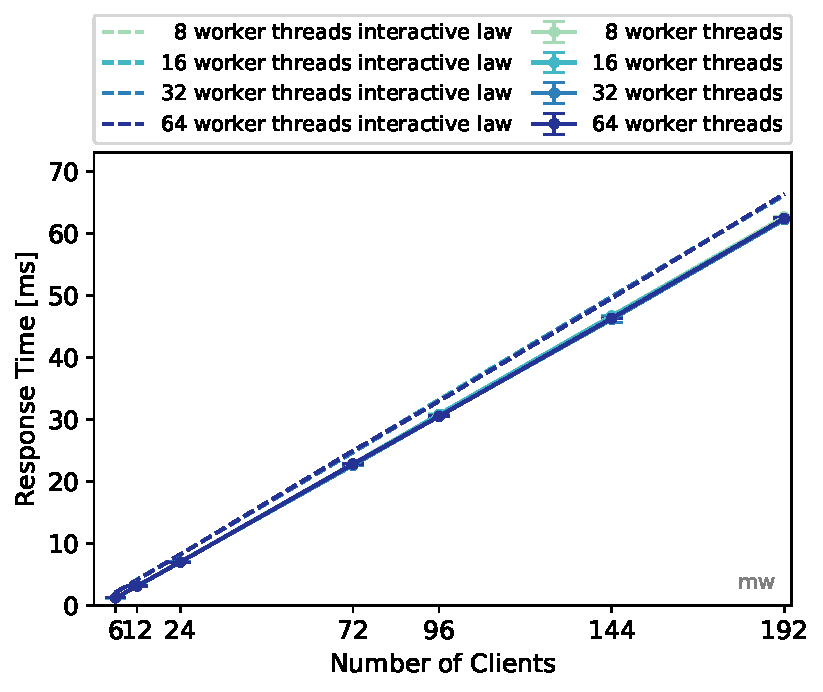
\includegraphics[width=\linewidth]{data/exp32_ro_rt_nc_w.pdf}
	\end{subfigure}%
	\caption{read-only workload}\label{exp32_ro_tp_nc}
\end{subfigure}
\\[1ex]
\begin{subfigure}{\linewidth}
	\begin{subfigure}[b]{.49\linewidth}
		\centering
		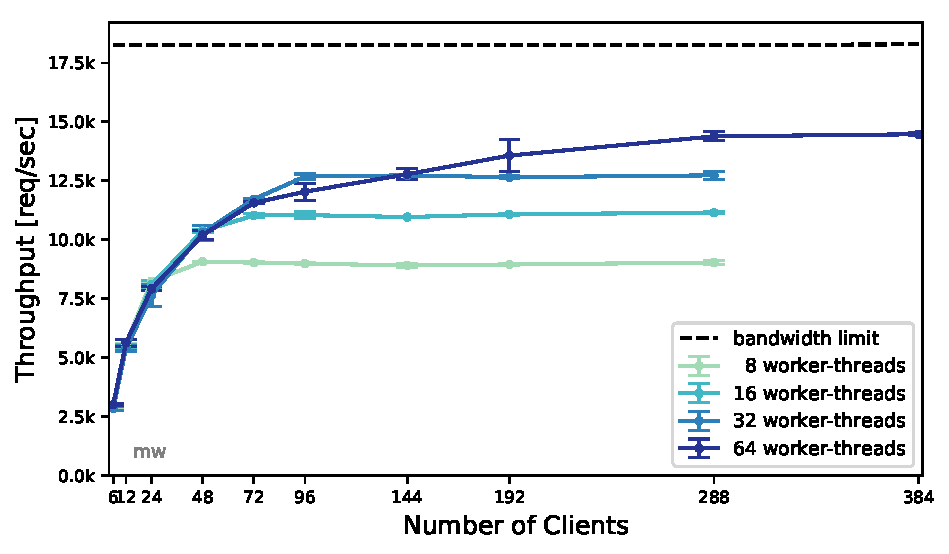
\includegraphics[width=\linewidth]{data/exp32_wo_tp_nc_w.pdf}
	\end{subfigure}\hfill
	\begin{subfigure}[b]{.49\linewidth}
		\centering
		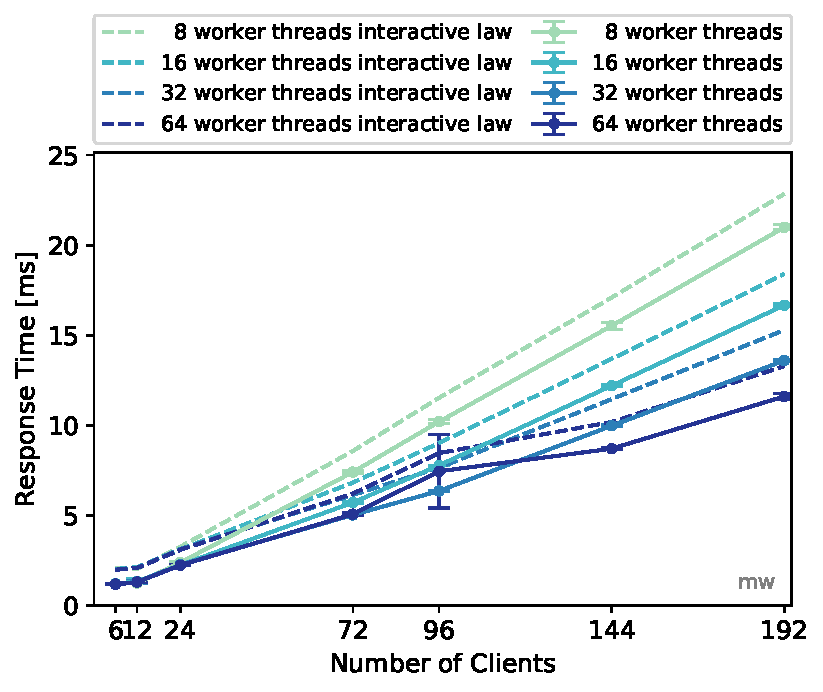
\includegraphics[width=\linewidth]{data/exp32_wo_rt_nc_w.pdf}
	\end{subfigure}%
	\caption{write-only workload}\label{exp32_wo_tp_nc}
\end{subfigure}
\caption{Throughput and response time for the system with 2 MWs as a function of number of clients. The sample standard deviation over the experiment repetitions is used as the error metric.}
\end{figure}


\subsubsection{Explanation}

\paragraph{Read-Only Workload}

As in the setting with 1 MW, the read-only workload is bound by the upload bandwidth of the server. Since the bottleneck is not related to the MW, it is no surprise that adding an additional MW does not change the observed behaviour and the throughput saturation is still reached at 6 clients independent of the number of workers (Fig. \ref{exp32_ro_tp_nc}). The response time also shows the same behaviour as in the case with 1 MW for the identical reasons.

However considering the internal MW measurements, there are a few differences.
Since the two MWs share the workload, each MW has only half of the clients.
Thus requests are only starting to be queued up in the request queue when there are two times more clients than workers per MW (Fig \ref{exp32_ro_q}).
The same holds for the server service times that start becoming constant in the number of clients when there are more than two times more clients than worker-threads due to the same reasons as outlined in section \ref{exp31}. 
The trade-off between queue waiting time and server service time as the dominating components of the response time is also evident in the setting with 2 MWs (Fig. \ref{exp32_ro_rtcomp}) and so the number of workers still does not influence the total response time but it influences in which part of the system the requests are queued.


\begin{figure}[H]
	\begin{subfigure}[b]{.33\linewidth}
		\centering
		\includegraphics[width=\linewidth]{data/exp32_ro_queue_nc_w.pdf}
		\caption{}\label{exp32_ro_q}
	\end{subfigure}\hfill
	\begin{subfigure}[b]{.33\linewidth}
		\centering
		\includegraphics[width=\linewidth]{data/exp32_ro_sst_nc_w.pdf}
		\caption{}\label{exp32_ro_sst}
	\end{subfigure}\hfill
	\begin{subfigure}[b]{.33\linewidth}
		\centering
		\includegraphics[width=\linewidth]{data/exp32_ro_rt_component_w.pdf}
		\caption{}\label{exp32_ro_rtcomp}
	\end{subfigure}
	\caption{Queue length and server service timeas a function of the number of clients and client response time component analysis for 144 clients  in a read-only workload with 2 MWs.}
\end{figure}
\vspace{-8mm}
\paragraph{Write-Only Workload}

In the write-only workload the system with 2 MWs behaves in a similar way as the system with 1 MW. 
As shown in figure \ref{exp32_wo_util_nc} the bottleneck remains the number of worker-threads that are waiting for a server response. 
However, the baseline without middleware suggests that for 72 clients the throughput saturation is reached. This means that using more than 72 workers in total does not lead to a higher throughput.
The server service time still depends only on the number of busy worker-threads (Fig. \ref{exp32_wo_rtcomp_nc}).
However, by adding an additional MW the total number worker-threads in the system is multiplied by two and hence the maximal throughput achieved is higher for the same number of worker-threads per MW.
For 8 worker-threads per middleware the point of saturation is reached with 48 clients, for 16 workers with 72 clients, for 32 workers with 96 clients and for 64 workers with 192 clients.

The collected data indicates that the total number of worker-threads in the system is the decisive factor for performance up to the point where the total number of workers reaches the saturation of the server.
So essentially the system with 2 MWs has a similar performance to the system with 1 MW with two times as many worker-threads. (i.e. system with two middlewares with 32 workers per MW has approximately the same performance as the system with 1 MW and 64 worker-threads)
This results from the fact that neither the net-thread nor the middleware VM network bandwidth is the bottleneck and so by duplicating the middleware VM the only performance gain is the consequence of more worker-threads in the system.

The total number of worker-threads in the system affect the performance because the server service time depends only on the number of worker-threads that are sending requests concurrently (Fig. \ref{exp31_wo_queue_sst_nc} and \ref{exp32_wo_queue_sst_nc}).
Consequently each request needs to wait in the queue for approximately the same time and hence the total response time is the same leading to the same throughput in systems with the identical number of total worker-threads (Fig. \ref{exp31_wo_tp_nc} and \ref{exp32_wo_tp_nc}).
The system with 1 MW has on average two times as many requests in the queue compared to each queue in the system with 2 MWs 
but the total number of requests in the whole system that are waiting in a middleware queue is the same when the total number of workers is identical (Fig. \ref{exp31_wo_queue_sst_nc} and \ref{exp32_wo_queue_sst_nc}).
\vspace{-2mm}

\begin{figure}[H]
	\begin{subfigure}[b]{.499\linewidth}
		\centering
		\includegraphics[width=\linewidth]{data/exp32_wo_queue_nc_w.pdf}
	\end{subfigure}\hfill
	\begin{subfigure}[b]{.499\linewidth}
		\centering
		\includegraphics[width=\linewidth]{data/exp32_wo_sst_nc_w.pdf}
	\end{subfigure}\hfill
	\caption{Queue length per MW and server service time per request in a write-only workload with 2 MWs. Boths graph show the sample standard deviation over the repetitions as error metric.}\label{exp32_wo_queue_sst_nc}
\end{figure}

\begin{figure}[H]
	\begin{subfigure}[b]{.499\linewidth}
		\centering
		\includegraphics[width=\linewidth]{data/exp32_wo_util_nc_w16.pdf}
		\caption{16 worker-threads}
	\end{subfigure}\hfill
	\begin{subfigure}[b]{.499\linewidth}
		\centering
		\includegraphics[width=\linewidth]{data/exp32_wo_util_nc_w64.pdf}
		\caption{64 worker-threads}
	\end{subfigure}\hfill
	\caption{Utilization $\frac{\text{busy time}}{\text{total time}}$ as a function of number of clients in a write-only workload with 2 MWs.}\label{exp32_wo_util_nc}
\end{figure}

\begin{figure}[H]
	\begin{subfigure}[b]{.499\linewidth}
		\centering
		\includegraphics[width=\linewidth]{data/exp32_wo_component_nc_w16.pdf}
		\caption{16 worker-threads}
	\end{subfigure}\hfill
	\begin{subfigure}[b]{.499\linewidth}
		\centering
		\includegraphics[width=\linewidth]{data/exp32_wo_component_nc_w64.pdf}
		\caption{64 worker-threads}
	\end{subfigure}\hfill
	\caption{Response time components as a function of number of clients for SET requests with 2 MWs.}\label{exp32_wo_rtcomp_nc}
\end{figure}


\subsection{Summary}

\begin{center}
	{Maximum throughput for one middleware.}
	\begin{tabular}{|l|p{2cm}|p{2cm}|p{2cm}|p{2cm}|}
		\hline                                & Throughput [ops/sec] & Response time [ms] & Average time in queue [ms] & Miss rate \\ 
		\hline Reads: Measured on middleware  &                 2814 &                1.2 &                        0.1 & 0.0       \\ 
		\hline Reads: Measured on clients     &                 2780 &                2.2 &                        n/a & 0.0       \\ 
		\hline Writes: Measured on middleware &                12030 &                9.8 &                        4.6 & n/a       \\ 
		\hline Writes: Measured on clients    &                12144 &                11.8 &                       n/a & n/a       \\ 
		\hline 
	\end{tabular}
\end{center}

\begin{center}
	{Maximum throughput for two middlewares.}
	\begin{tabular}{|l|p{2cm}|p{2cm}|p{2cm}|p{2cm}|}
		\hline                                & Throughput [ops/sec] & Response time [ms] & Average time in queue [ms] & Miss rate \\ 
		\hline Reads: Measured on middleware  &                 2869 &                1.2 &                        0.1 & 0.0       \\ 
		\hline Reads: Measured on clients     &                 2827 &                2.1 &                        n/a & 0.0       \\ 
		\hline Writes: Measured on middleware &                13569 &               12.8 &                        3.5 & n/a       \\ 
		\hline Writes: Measured on clients    &                13776 &               14.0 &                        n/a & n/a       \\ 
		\hline 
	\end{tabular}
\end{center}


\paragraph{Analysis}

As shown in sections \ref{exp31} and \ref{exp32} the read-only workload is independent of the number of middlewares in the setup with one server VM and thus in the follwing results are summarized for both systems together.
The optimal number of clients for the read-only workload is somewhere in between 6 and 12 clients but the configuration with 12 clients is already strongly affected by the bandwidth bottleneck and results in a response time that is almost two times as long with only a small gain in throughput. So under the evaluated configurations the maximum throughput is achieved with 6 clients and is independent of the number of worker-threads. Thus there is no point in using more than 8 workers. 
There are no misses because before every experiment \emph{memcached} is initialized with all keys and thus misses have no influence on the response time. Since in the optimal configuration the number of worker threads is greater than the number of clients, the queue basically remains empty and consequently the average time of a request in the queue is a negligible factor in the response time.

For a write-only workload the maximum throughput  in the system with a single middleware is achieved with 144 clients and 64 middleware worker-threads. In the system with two middlewares the point of throughput saturation is reached at 192 clients when using 64 worker-threads per middleware. The maximum throughput of the system involving two middlewares comes close to the maximum throughput of 14000 ops/sec recorded in the baseline without a middleware\footnote{The experiments of this section were run after restarting the VMs used in the baseline without middleware and so the measurements are only approximately comparable.} 
It can be concluded that the overhead of using a middleware in a write-only workload with a single server is minimal, because the baseline without MW poses an upper bound on what can be achieved for a write-only workload.

Since in both setups there are more clients than worker-threads, requests usually spend some time waiting in the queue. However, the additionally gained throughput outweighs the longer response time incurred by this waiting time.
The difference between response time measurements on the client and the middleware is between 1 and 2 milliseconds for both workloads which is consistent with the round trip time measurements between the involved VMs. The small difference in throughput measurements can be explained by the exclusion of warm up and cooldown phase in the middleware. 

\paragraph{One middleware vs. two middlewares}

For the read-only workload having one or two middlewares does not make a difference because the server VM network bottleneck is not affected by the number of middlewares in the system.

For a write-only workload the maximal throughput achieved with two middlewares is higher than with a single middleware but  this is only an indirect consequence of having an additional middleware because the maximum total number of workers evaluated in the two systems is different and this is the important parameter for the performance as outlined in section \ref{exp32}. The maximal throughput in the system with two middlewares is achieved with 64 worker-threads per middleware and thus 128 workers in total. The configuration with a single middleware and 128 worker-threads was not evaluated but the data indicates that this could produce a similar performance assuming the middleware VM does not start to get a problem with context switches or another effect slowing down individual threads.

\paragraph{Key take-away messages}
\begin{itemize}
	\vitemsep
	\item the number of worker-threads is the main factor for performance in a write-only workload
	\item with two middlewares and the resulting 128 worker-threads, the maximal throughput of the baseline without middleware is almost reached
	\item round trip time between client and middleware VM is varying between 1 and 2 milliseconds
\end{itemize}

\end{document}